\begin{table}[h]
	\small
	\caption{}
	\label{table:}
	\begin{tabular}{p{0.3\width}}
	\graytable
	\toprule
	\midrule
	\bottomrule
	\end{tabular}
\end{table}




\section{Материалы и методы}
\subsection{Материалы}



\subsubsection{Использованные штаммы микроорганизмов}
\label{subsec:strains}

Штаммы дрожжей и бактерий описаны в таблице~\ref{table:strains}.

Использованные родительские штаммы были взяты из коллекции лаборатории. Созданные штаммы также архивировали, суспендируя свежие клетки в 1\,мл стерильного 20\%\,глицерина, затем хранили при -70 ºС.

Штамм cdc53-1 -- термочувствительный мутант, который растет и делится при пермесивной температуре 25°C, но аррестуется в фазе G\textsubscript{0} при 37°C \cite{mathias_cdc53p_1996}. Белок Cdc53 -- компонент убиквитин-лигазной системы, которая направляет фосфорилированные циклины  G\textsubscript{0} (Cln1, Cln2, Cln3) на протеасомную деградацию \cite{willems_cdc53_1996}. Точнее, это каркасный белок различных комплексов Cdc34/Skp1/F-box, которые участвуют в регуляции клеточного цикла и синтеза метионина \cite{patton_cdc53_1998}, а мутация cdc53-1, возможно, даже нарушает целосность клеточной стенки дрожжей \cite{varelas_cdc34/scf_2006}.

\begin{table}[p]
	\small
	\caption{Описание штаммов дрожжей и бактерий, использованных в работе.}
	\label{table:strains}
	\begin{tabular}{ p{0.25\width - \tabcolsep} p{0.65\width - 2\tabcolsep}  p{0.1\width - \tabcolsep}}
		\graytable
		\toprule
		Название штамма & Описание & Источ-ник \\ 
		\midrule
		
		\multicolumn{3}{l}{ \textit{Saccharomyces cerevisiae} }\\
		\invisiblerule
		W303 &
			MAT\textbf{a} ade2-101 his3-11 trp1-1 ura3-52 can1-100 leu2-3,112, GAL, psi+ &
			$^1$ \\  \invisiblerule
		cdc53-1 &
			MAT\textbf{a} ade2-1 his3-11 trp1-1 ura3-52 can1-100 leu2-3,112,15 cdc53-1 &
			$^1$ \\  \invisiblerule
		W303-1a::URA3 &
			 MAT\textbf{a} ade2-101 his3-11 trp1-1 URA3 can1-100 leu2-3,112, GAL, psi+&
			$^1$ \\  \invisiblerule
		диплоид &  
			diploid ade2-101 his3-11 trp1-1 ura3-52 can1-100 leu2-3,112, GAL, psi+ 
			& $^1$\\   \invisiblerule
		W303/αSyn &  W303-1a, плазмида p426GALaSynGFP & $^2$\\  \invisiblerule
		cdc53-1/αSyn &  cdc53-1, плазмида p426GALaSynGFP & $^2$ \\  \invisiblerule
		W303/αSyn/LEU2 &  W303-1a, плазмиды p426GALaSynGFP и YEp13 & $^2$ \\  \invisiblerule
		cdc53-1/αSyn/LEU2 &  cdc53-1, плазмиды p426GALaSynGFP и YEp13 & $^2$\\  \invisiblerule
		W303::URA3/LEU2& W303-1a::URA3, плазмида YEp13 & $^2$ \\
		
		\midrule
		\multicolumn{3}{l}{\textit{Escherichia coli} }\\ \invisiblerule
		E.coli XL1 Blue &
		recA1 endA1 gyrA96 thi-1 hsdR17 supE44 relA1 lac [F' proAB lacI\textsuperscript{q}Z$\Delta$M15 Tn10 (Tet\textsuperscript{r})]&
		\scriptsize{EvroGen\texttrademark} \\
		
		
		\bottomrule
	\end{tabular}
	\begin{tabular}{p{1\width}}
			$^1$ коллекция лаборатории \\
			$^2$ штаммы были получены из приведенных введением плазмид
			\\
	\end{tabular}
	
\end{table}





\subsubsection{Плазмиды и библиотеки} 
\label{subsec:libs}

Плазмиды, использованные в данной работе, охарактеризованы в таблице~\ref{table:plasmids}. 

Плазмида p426GALaSynGFP \cite{outeiro_yeast_2003} использовалась для экспрессии и изучения гибридного белка -- α-синуклеина, слитого с GFP. Карта плазмиды приведена на рисунке~\ref{fig:plasmid}.


\begin{table}[p]
	\small
	\caption{Плазмиды, использованные в работе.}
	\label{table:plasmids}
	\begin{tabular}{ 
		p{0.3\width - \tabcolsep}
		p{0.55\width - 2\tabcolsep} 
		p{0.15\width - \tabcolsep} }
	\graytable
	\toprule
	Плазмида & Описание & Источник \\ \midrule

	p426GALaSynGFP  &
		2$\mu$, URA3, ampR, экспрессия α-синуклеина-GFP&
		\cite{outeiro_yeast_2003} \\
	pYES-DA-6 &
		2$\mu$, URA3, ampR & $^1$ \\
	pYES2 &
		2$\mu$, URA3, ampR & $^1$\\	
	YEp13 &
		2$\mu$, LEU2, ampR & $^1$ \\
	pRS314 &
		CEN/ARS, TRP1, ampR & $^1$\\

	\bottomrule
	\end{tabular}
	\begin{tabular}{p{1\width}}
			$^1$ коллекция лаборатории \\
	\end{tabular}
	
\end{table}

\begin{figure}[p]
	\centering
	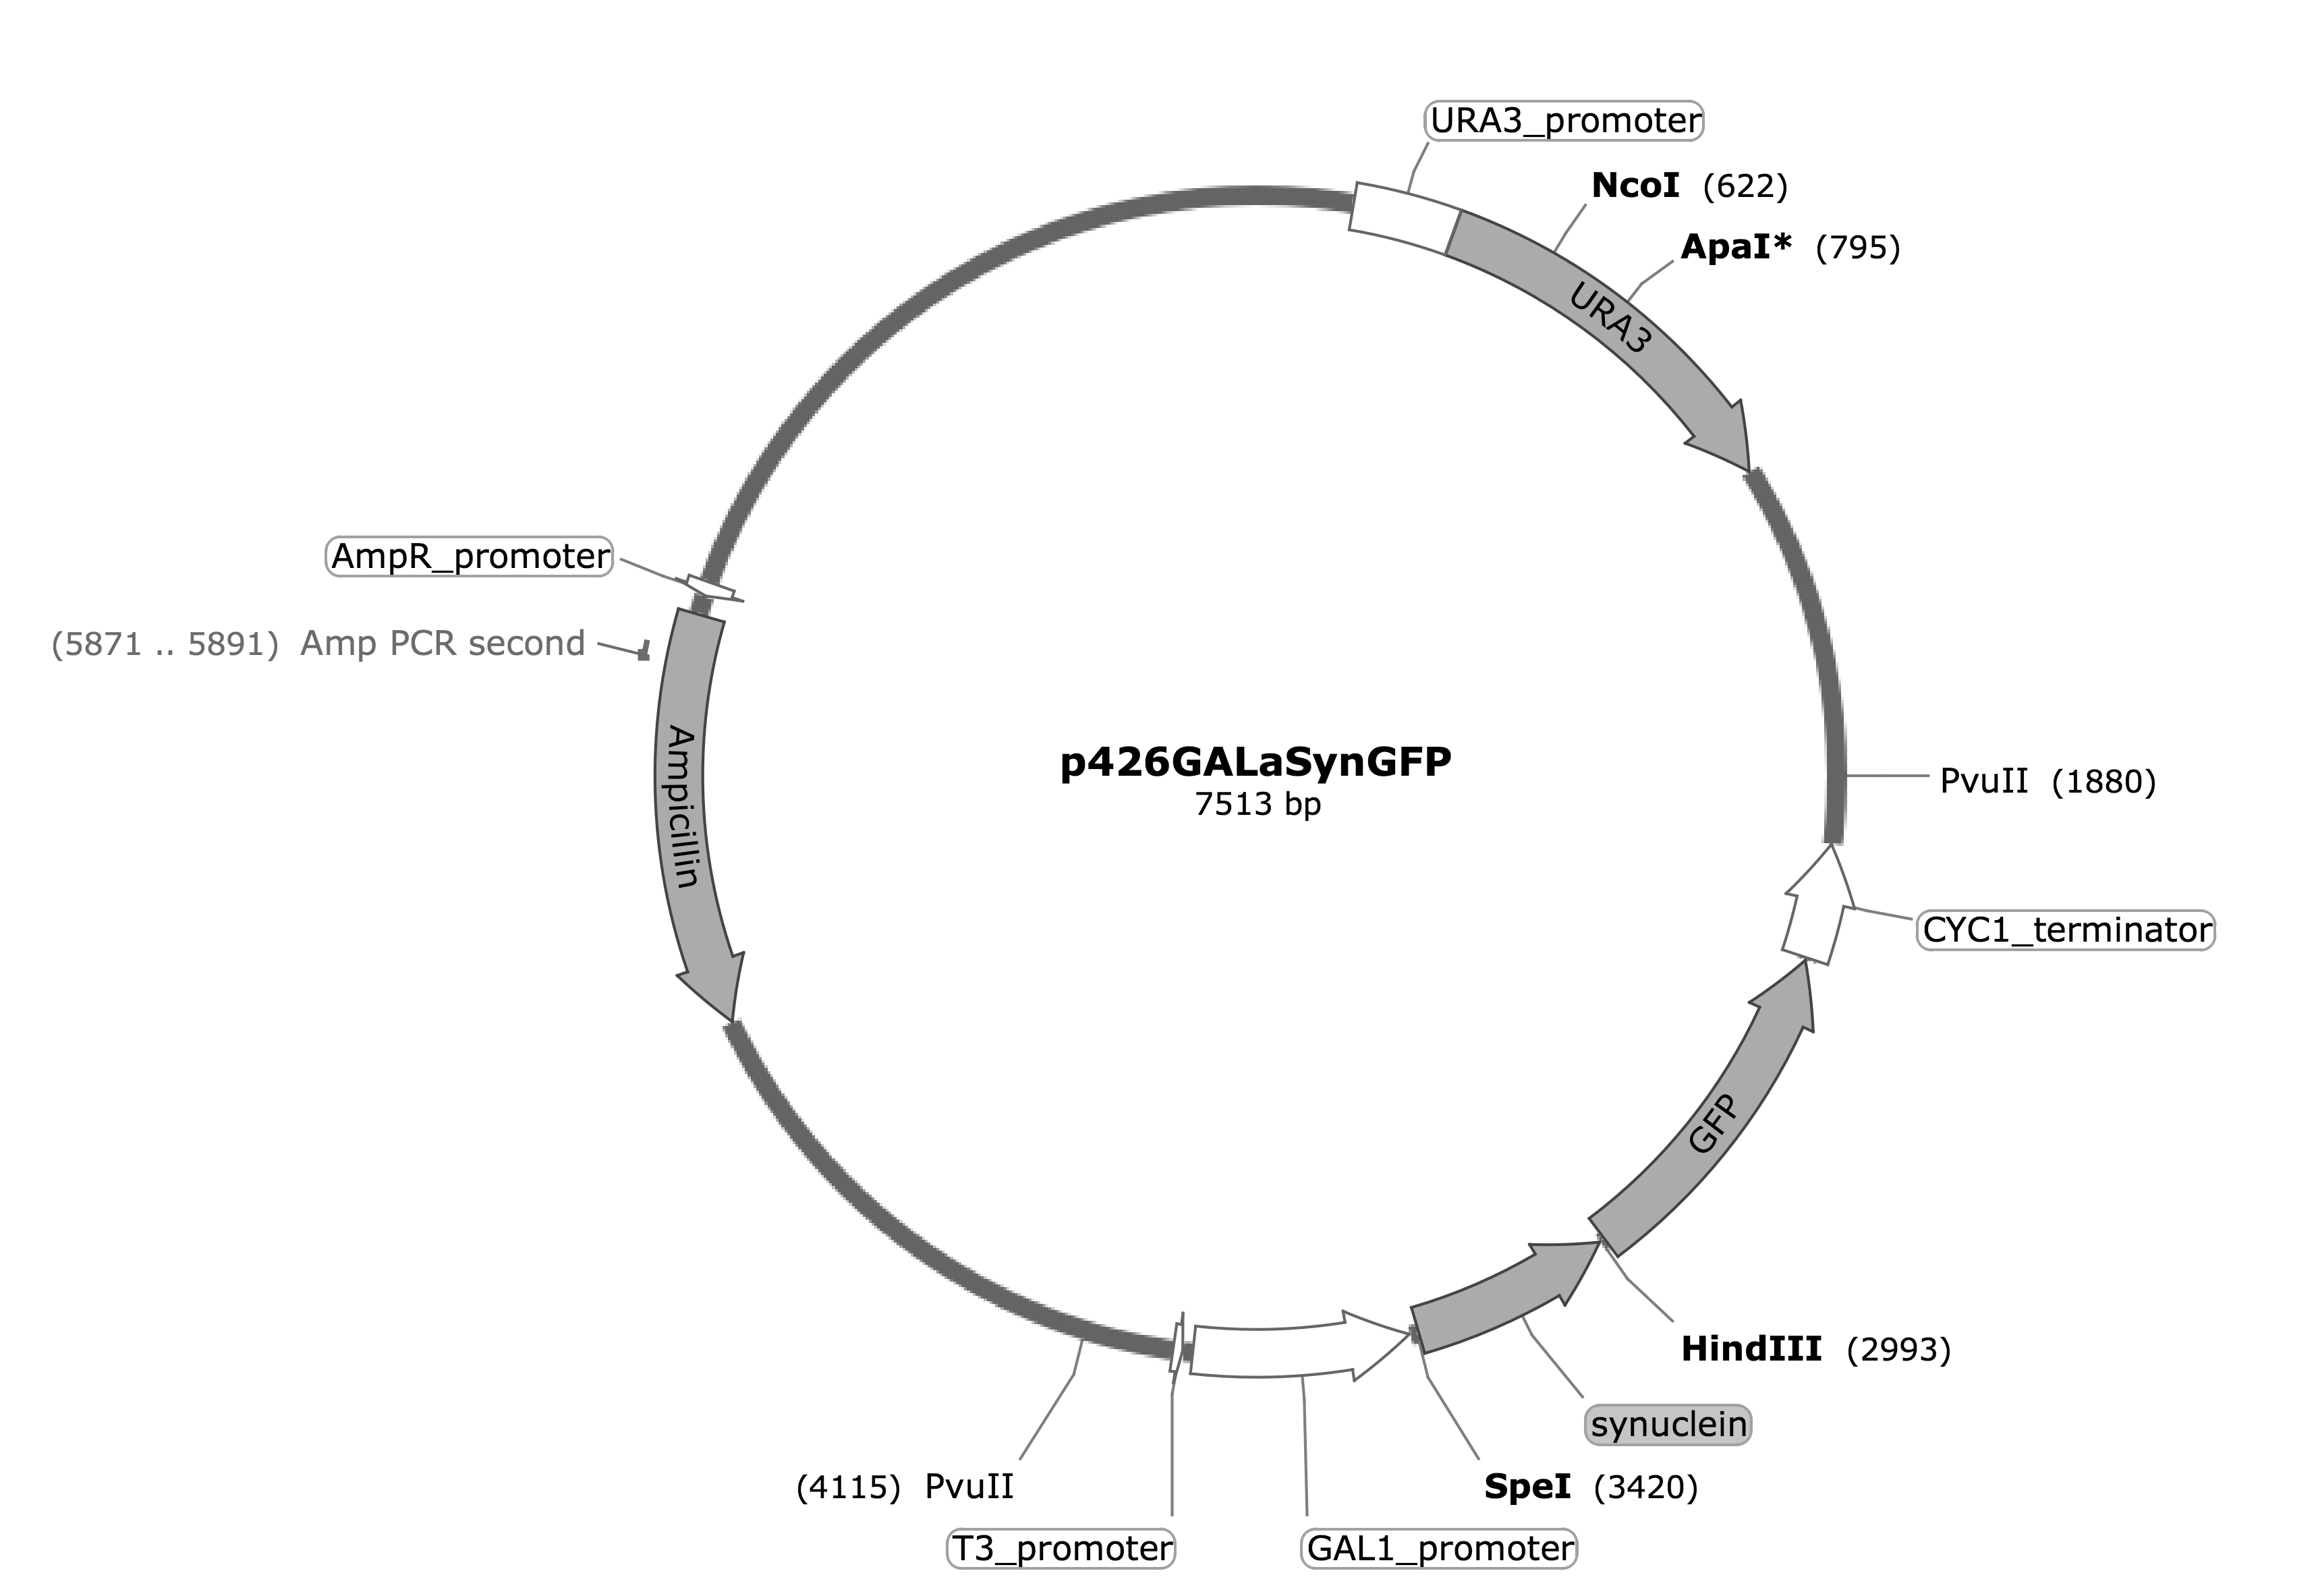
\includegraphics[width = 0.85\textwidth]{pics/p426GALaSyn_Map}
	\caption{Карта плазмиды p426GALaSynGFP, которая использовалась для экспрессии гибридного белка α-синуклеина-GFP в дрожжах. \gray{Точная нуклеотидная последовательность плазмиды нам была не известена, данная карта составлена на основе описания \cite{outeiro_yeast_2003} } }
	\label{fig:plasmid}	
\end{figure}


Геномные библиотеки, которые использовались для скринина, представлены в таблице~\ref{table:libs}.

Сверхэкспрессионная --  эписомальная, мультикопийная библиотека YEp13\,lib, используется в виде плазмид.
Делеционная -- библиотека lib25 \cite{burns_large-scale_1994}. Lib25 представляет из себя геномную библиотеку дрожжей, лигированную в вектор pHSS6, в которую далее был встроен транспозон mini-Tn3::LEU2, использовалась в виде продукта рестрикции по уникальному сайту NotI(см. \ref{sec:restriction}).

\begin{table}[p]
	\small
	\caption{Геномные библиотеки, использованные в работе.}
	\label{table:libs}
	\begin{tabular}{p{0.4\width - \tabcolsep}p{0.3\width - 2\tabcolsep}p{0.3\width - \tabcolsep}}
	\graytable
	\toprule
	&YEp13 lib& Lib25 \\
	\midrule
	Тип & 
		эпимсомальная, мультикопийная, оверэкспрессионная & 
		делеционная \\ \thinrule
	Исходный вектор & YEp13 & pHSS6\\ \thinrule
	Исходный размер вектора & 10.7\,kb & 2,5\,kb\\ \thinrule
	Размер фрагментов геномной ДНК дрожжей & 5-20\,kb & 1,9-3,5\,kb (в среднем 3kb)\\ \thinrule
	Маркёры & LEU2, ampR & LEU2, ampR \\ \thinrule
	
	Количество клонов для покрытия генома дрожжей & $1.0\times10^4$ & $3.0\times10^4$ \\ \thinrule
	Число независимых рекомбинантов (вариантов вектора) & $8.2\times10^4$ & $>10^5$ \\ \thinrule
	Источник & 
		\footnotesize{ \textit{Saccharomyces cerevisiae} (ATCC\textregistered 37323\texttrademark)} &
		\cite{burns_large-scale_1994} \\
	\bottomrule
	\end{tabular}
\end{table}





\subsection{Культивирование}
\subsubsection{Условия культивирования}
Микроорганизмы растили на питательных средах различного состава (таблица~\ref{table:mediums}) в термостате (на твердой агаризованной среде на чашках Петри) или термостатируемой качалке (на жидкой среде в колбах и 50 мл пробирках типа «Falkon», обязательное перемешивание 250 rpm). Оптимальная температура роста для дрожжей --  30 ºС (для не термочувствительных штаммов) или  25 ºС (для термочувствительных мутантов cdc53). Бактерии растили при 37 ºС.


\subsubsection{Среды для культивирования}
Питательные среды, использовавшиеся для культивации дрожжей и бактерий, перечислены в таблице~\ref{table:mediums}. Бактерии растили в LB. Дрожжи дикого типа растили на натуральной среде (YPD), мутантов, содержащих плазмиды с селективными маркёрами -- на соответствующих синтетических селективных средах (YNB).

В твердые среды добавлялся агар. Среды стерилизовали автоклавированием при 2 атм. 121 ºC в течение 50 минут. Растворы сахаров автоклавировали отдельно, затем смешивали со средой. Антибиотики добавляли в среды после автоклавирования. 

\begin{table}[p]
	\footnotesize
	\caption{Состав сред для культивирования}
	\label{table:mediums}
	\begin{tabular}{ p{0.3\width - \tabcolsep} p{0.55\width - 2\tabcolsep} p{0.15\width - \tabcolsep} }
	\graytable
	\toprule
	Название & Состав & \\
	\midrule
	LB & 
		LB \scriptsize (триптон 10г, дрожжевой экстракт 5г, NaCl 10г)& 25 г/л\\
		& (агар) & 20 г/л\\

	\thinrule
	LB Amp & 
		LB & 25 г/л\\
		& (агар) & 20 г/л\\
		& ампицилин & 0.1 г/л\\
	\thinrule
	SOC & 
		LB & 25 г/л \\
		&МgCl\textsubscript{2} & 5 мМ\\
		&MgSO\textsubscript{4} & 5 мМ\\
		&глюкоза& 10 г/л\\
	YPD & 
			дрожжевой экстракт & 10 г/л \\ 
			& пептон  & 20 г/л\\
			& D-глюкоза & 20 г/л \\
			& (агар) & 20 г/л \\
			
	\thinrule
	YNB selective D/GAL & 

			YNB (yeast nitrogen base) &  6.6 г/л\\
			&селективная аминокислотная добавка (табл.~\ref{table:dropout}) & ...\\
			&D-глюкоза / D-галактоза & 20 г/л \\
			&(агар) & 20 г/л \\


	\bottomrule
	\end{tabular}
\end{table}

\begin{table}[p]
	\footnotesize
	\caption{Аминокислотные добавки для селективных сред}
	\label{table:dropout}
	\begin{tabular}{p{0.3\width - \tabcolsep} p{0.6\width - 2\tabcolsep} p{0.1\width - \tabcolsep}}
	\graytable
	\toprule
	Селективная среда & Аминокислотная добавка & \\
	\midrule
	-ura & Yeast Synthetic Drop-out Medium Supplements without (YSDMS w/o) uracil & 1.92 г/л\\
	\thinrule
	-leu & YSDMS w/o leucine  & 1.6 г/л\\
	\thinrule
	-ura-leu & YSDMS w/o histidine, leucine, tryptophan and uracil  & 1.4г/л \\
		& L-histidine & 20 мг/л \\
		& L-tryptophan & 20 мг/л \\
		\\
	
	\bottomrule
	\end{tabular}
\end{table}



\subsection{Молекулярно-биологические методы}


\subsubsection{Подготовка компетентных бактериальных клеток}
\label{subsec:bac_comp}

Компетентные клетки для электропорации готовили из электрокомпетентных клеток EvroGen\texttrademark E.coli XL1 Blue.
 
\begin{enumerate}[nolistsep]
	\item Клетки растили ночь в больших колбах (3-4 штуки) в LB при 30ºC и перемешивании 200\,rpm. Заранее охлаждали mQ и 10\% глицерин. 
	\item Через 12 часов измеряли оптическую плотность клеток при 595\,нм и доводили ее до 0.1-0.2 о.е. Растили при температуре 18ºC и перемешивании 6 часов в тех же колбах в LB (по 200\,мл).
	\item  Центрифугированили при температуре 4ºC  2200\,g 7\,мин. Промывали клетки холодной (4ºC) mQ (по 20 мл) 3 раза. Промывали клетки 10\% глицерином (20\,мл). 
	\item Ресуспендировали клетки в остатках глицерина (около 2\,мл). Аликвотировали в холодные пробирки по 50\,млкл. Замораживали в жидком азоте. Хранили при -70ºC.

\end{enumerate}

\subsubsection{Трансформация бактериальных клеток}
\label{subsec:bac_tranform}

Трансформацию бактериальных клеток \emph{Escherichia coli} проводили методом электропорации.

Для трансформации аликвоту компетентных клеток оттаивали во льду 20\,минут, добавляли ДНК, смесь перемешивали, инкубировали во льду (4ºC 10\,мин) и переносили в холодную кювету для электропорации, подвергали действию электрического разряда (1800\,В), после чего добавляли 500\,мкл SOC, инкубировали (37 ºС 60 мин при перемешивании 700\,rpm), сеяли на чашку(чашки) с селективной средой и растили ночь в термостате при 37 ºС.

\subsubsection{Выделение плазмидной ДНК из бактерий}
\paragraph{Выделение плазмид}
\label{subsec:bac_plasm_pur}
\begin{enumerate}[nolistsep]
	\item Для выделения плазмид одну колонию с чашки транформированных бактерий или небольшое число клеток из архива суспендировали в 2-3\,мл жидкой селективной среды и растили ночь при 37ºС.
	\item Ночную культуру охлаждали  в  течение  15\,мин  на  льду, центрифугировали (1400\,g 2\,мин), ресуспендировали в 250\,мкл охлажденной деионизованной воды и переносили на лед. 
	\item Добавляли 500\,мкл лизирующего буфера В (0,2\,M NaOH, 1\%\,SDS), аккуратно перемешивали, инкубировали (25ºС 3\,мин).
	\item Затем добавляли 350\,мкл нейтрализующего буфера С (5М ацетат калия, pH 7), встряхивали,  инкубировали (25ºС 15\,мин), затем центрифугировали (17000\,g 5\,мин). 
	\item Отбирали супернатант, содержащий плазмидную ДНК. 
	\item Добавляли 0,6 объема изопропанола, инкубировали во льду (4ºС 10\,мин), центрифунировали (17000\,g 5\,мин).
	\item Убирали супернатант, днк в осадке. Добавляли 500\,мкл mQ, 300\,мкл 9\,М ацетата аммония (NH\textsubscript{4}Ac), инкубировали в морозилке (-20ºС 5\,мин) и затем в холодильнике (4ºС 15\,мин), центрифунировали (17000\,g 5\,мин).
	\item Отбирали супернататант, добавляли 0,6 объема изопропанола, инкубировали во льду (4ºС 10\,мин), центрифунировали (17000\,g 5\,мин).
	\item Промывали ДНК этанолом: сливали изопропанол, добавляли 0,2,\,мл 70\%\,этанола, центрифунировали (2500\,g 2\,мин), убирали этанол.
	\item Подсушивали и растворяли в 100\,мкл деионизированной воды с небольшим добавлением РНКазы H(0,1\,мкл на 1\,мл воды).

	\end{enumerate}
	
\paragraph{Выделение плазмидных библиотек}
\label{subsec:bac_plasm_kit}
Для амплификации библиотек трансформированные бактерии высевали на большое число селективных чашек (10), растили ночь при температуре 37ºС. Контролировали число полученных клонов -- оно должно было превышать число клонов, необходимых для покрытия генома данной библиотеков (табл.~\ref{table:libs} и раздел \ref{subsec:libs}). Затем смывали колонии водой, выделяли и переосаждали плазмидную ДНК с помощью набора QIAGEN\textregistered Plasmid Purification Midi Kit.

\subsubsection{Переосаждение ДНК}
\label{subsec:dna_prec}

Переосаждение ДНК из раствора проводили на льду следующим образом: подсаливали раствор до 0.2\,М NaCl, добавляли 2.5\,объема спита EtOH 100\%,  инкубировали (30\,мин), центрифугировали (17000\,g 5\,мин), сливали супернатант, добавляли спирт EtOH 70\%, центрифугировали (17000\,g 5\,мин), сливали супернатант, высушивали, растворяли ДНК в воде.

\subsubsection{Обработка ДНК эндонуклеазами рестрикции} \label{sec:restriction}
	Для анализа различных образцов ДНК проводили рестрикцию различными эндонуклеазами рестрикции. Рестрикционную смесь готовили на основе деионизированной воды, десятикратного рестрикционного буфера, образца ДНК, рестриктазы.
	
	Рестрикцию плазмид или библиотек для последующего анализа на геле проводили в объеме 10\,мкл, используя 1-2\,мкл плазмиды и 0.2\,мкл фермента в течение 1-2\,часов при 37ºС.
	
	Рестрикцию делеционной библиотеки lib25 для дальнейшего использования проводили в объеме 120\,мкл, используя 30\,мкл библиотеки и 5\,мкл фермента NotI в течение 2-3\,часов при 37ºС с последующим переосаждением.

\begin{table}[!h]
	\small
	\caption{Эндонуклеазы рестрикции, использованные для анализа плазмид}
	\label{table:}
	\begin{tabular}{
		p{0.4\width - \tabcolsep}
		p{0.6\width - \tabcolsep}}
	\graytable
	\toprule
	Плазмида & Анализ рестриктазами\\
	\midrule
	p426GALaSynGFP & ApaI, HindIII, NcoI, PvuII, SpeI (рис.~\ref{fig:plasmid}) \\
	библиотека YEp13 & Eco32(EcoRV) (0.96, 3.3 kbp, inserts)\\ 
	делеционная библиотека lib25 & NotI(unique) \\
	pYes-DA-6 & Eco32(EcoRV) (unique)\\
	YEp13 &  Eco32(EcoRV) (0.96, 3.3, 6.4 kbp) \\
	pRS314 & Eco32(EcoRV) (1.2, 3.6 kbp) \\

	\bottomrule
	\end{tabular}
\end{table}	

\subsubsection{Горизонтальный гель-электрофорез ДНК}
\label{subsec:gel}
Для определения количества и размеров фрагментов ДНК использовали горизонтальный электрофорез в агарозном геле в присутствии бромистого этидия. Использовали гель на основе буфера ТАЕ (40мМ трис-ацетат (рН\,8.2), 20\,мМ ацетат натрия, 2\,мМ ЭДТА) с 1\% агарозы и бромистым этидием (0.5\,мг/мл) . Наносимые образцы предварительно смешивали с буфером для внесения (6x Loading Buffer - 0,25\%\,бромфеноловый синий, 0,25\%\,ксиленцианол, 30\%\,глицерин на воде).

Для рестрикционного анализа плазмид на гель наносили образец, обработанный рестриктазами, эквивалентное количество нативной ДНК, маркёры.

\subsubsection{Трансформация дрожжей}
\label{subsec:yeast_trans}
\begin{enumerate}[nolistsep]
	\item Клетки для трансформации в ночь освежали на твердой среде.
	\item Готовили свежий литий-ацетатный буфер (100\,мкл 1\,М ацетата лития, 10\,мкл 0,1\,М Трис-HCl pH 7,5, 2\,мкл 0.5\,М ЭДТА pH 8 на 1\,мл буфера).
	\item Суспендировали клетки в 200\,мкл литий-ацетатного буфера в 1,7\,мл эппендорфе, инкубировали (30ºС 15\,мин).
	\item Центрифугировали (2,5\,мин 350g), отбирали супернатант, ресуспендировали клетки в 70\,мкл литий-ацетатного буфера, инкубировали (30ºС 15\,мин).
	\item Добавляли 4\,мкл предваритально прокипяченой днк-носителя (днк спермы лосося, 10\,мг/мл), днк для трансформации, 120\,мкл 50\% полиэтиленгликоля PEG-4000, перемешивали пипетированием и инкубировали (30ºС 30\,мин).
	\item Подвергали тепловом шоку в водяной бане (42ºС 15\,мин).
	\item Высеивали на селективную чашку. 
\end{enumerate}



\subsubsection{ПЦР}
\label{subsec:pcr}

%Для проверки интеграции плазмид в геном, клоны, полученные в результате трансформации, анализировали с помощью  полимеразной цепной реакции (ПЦР).
%Отдельные колонии с трансформационной чашки подращивали в ночь на селективной среде.

ПЦР проводилась в тонкостенных эпиндорфах на 500\,мкл в объеме 20\,мкл. Состав смеси указан в таблице~\ref{table:pcrmix}. Смесь ПЦР в эппендорфах накрывалась слоем масла (1-2\,мм). ПЦР проводилась на приборе Терцик согласно программе в таблице~\ref{table:pcrprog}.

\begin{table}[H]
	\small
	\caption{Состав смеси ПЦР на одну пробу}
	\label{table:pcrmix}
	\begin{tabular}{p{0.4\width - \tabcolsep} p{0.6\width - \tabcolsep}}
		\graytable
		\toprule
		Использованный раствор &  Конечная концентрация \\
		\midrule
		mQ & до 20\,мкл\\ \verythinrule
		буфер для Taq-pol с KCl, 10$\times$ & 1$\times$\\ \verythinrule
		MgCl\textsubscript{2}  25 мМ & 2.5 мМ\\ \verythinrule
		праймеры & по 0.2 мкМ\\ \verythinrule
		смесь нуклеотидов dNTPS 20мМ & 0.2 мМ \\ \verythinrule
		TAQ-полимераза 5 U/мкл & 0.07-0.1 U/мкл\\ \verythinrule
		матрица & сверх объема смеси вносилось очень маленькое количество клеток, на кончике носика для пипетки\\ 
		\bottomrule
	\end{tabular}
\end{table}



\begin{table}[H]
	\small
	\caption{Программа, использованная для проведения ПЦР.}
	\label{table:pcrprog}
	\begin{tabular}{ >{\raggedleft\arraybackslash}p{0.3\width} p{0.01\width} l l}
		кипячение и разрушение клеточных стенок & &$T = 94ºC$ & $ 30''$ \\ \thinrule
		амплификация  -- 30$\times$ & $\begin{cases} \\  \\	\end{cases}  $ 
			&  \pbox{20cm}{$T = 94ºC $\\ $T = 55ºC $\\$T = 72ºC $ } 
			&\pbox{2cm}{$30''$\\ $30''$\\$3'$ $^1$} 
			\\ \thinrule
		&&$T = 72ºC$&$ 10'$  \\	
		\end{tabular}
		
		
		\begin{tabular}{p{1\width}}
			$^1$для повышения эффективности иногда использовали двух-стадийный ПЦР: на первых 10 циклах амлификации время элонгации составляло $4'$
			\\
	\end{tabular}

\end{table}



\begin{table}[H]
	\small
	\caption{Последовательности праймеров}
	\label{table:primers}
	\begin{tabular}{p{0.3\width - \tabcolsep}p{0.7\width - \tabcolsep}}
		\graytable
		\toprule
		Название & Последовательность \\
		\midrule
		URA3-C & GGC-CAT-GAA-GCT-TTT-TCT-TT \\
		URA3-200 & TGG-TTT-CAG-GGT-CCA-TAA-AG\\
		%Amp PCR & GGT-AAG-CCC-TCC-CGT-ATC-GTA\\
		Amp PCR second & GCT-TCT-TTT-ACT-TTC-ACC-AGC\\
		%T3 & AAT-TAA-CCC-TCA-CTA-AAG-GG\\
		%T7 & TAA-\\
		
		\bottomrule
	\end{tabular}
\end{table}

\subsection{Методы, использованные при проведении скрининга}
\subsubsection{Методы интеграции плазмид}
\label{subsec:integration}

Интеграцию плазмид p426GALaSynGFP, pYes-DA-6 осуществляли трансформацией дрожжей линейной плазмидой, обработанной рестриктазой на участке, который гомологичен некоторому участку в геному дрожжей.

Родительский штамм W303 содержал мутантный ген ura3-52, с котором расположен транспозон Ty1 \cite{rose_identification_1984}. Рестрикция плазмид проводилась внутри гена ura3. Таким образом, линеаризованная плазмида имела по краям участки гомологии с геномом, и, учитывая расположение мутации в ura3-52, после трансформации и гомологической рекомбинации могло приводить к появлению клонов с интегрированной в геном плазмидой.

Плазмиду p426GALaSynGFP обрабатывали рестриктазой ApaI, NcoI или обеими, плазмиду pYes-DA-6 -- рестриктазой Eco32.

Для проверки интеграции плазмид в геном, клоны, полученные в результате трансформации, анализировали с помощью  полимеразной цепной реакции (ПЦР). Отдельные колонии с трансформационной чашки подращивали в ночь на селективной среде.

Использовались две пары праймеров -- (I)URA3-200, URA3-C, которая давала бы фрагмент длиной ~1.2\,kbp с геномного гена URA3, если встраивание не произошло, (II)URA3-200, Amp PCR second, которая давала бы фрагмент ~1.2\,kbp с геномного фрагмента, включающего участок встроенной плазмиды и участок около гена URA3, если произошла интеграция.

В качестве дополнительного позитивного контроля для опытов с I парой праймеров ставили ПЦР со штамма W303/αSyn, который давал продукт амплификации длиной  ~1.2\,kbp. 

Было проанализировано 20 клонов для плазмиды p426GAlaSynGFP, 10 для плазмиды pYES-DA-6 с помощью ПЦР. Дополнительно, некоторые клоны были трансформировали оверэкспрессионной библиотекой. В результате клонов с встроившейся плазмидой и/или транформирующихся библиотекой найдено не было.



\subsubsection{Стратегии скрининга}
\label{subsec:screening_strats}

Для проведения скрининга штамм подращивали 12-18 часов (ночь) на селективной чашке с глюкозой. Проводили несколько параллельных трансформаций по литий-ацетатному протоколу с использованием библиотеки -- 5\,мкл оверэкспрессионной, или 10\,мкл делеционной (полученной из 15\,мкл исходной библиотеки рестрикцией и переосаждением). Два варианта послейдующих действий:

\paragraph{Скрининг с печатаньем}
\label{subsec:printing}
Трансформацию высевали на  селективную среду с глюкозой и подращивали 1-2 суток до появления мелких колоний (минимально видимых). Затем чашку перепечатывали на индуцирующую селективную среду и растили. 
  

\paragraph{Высевание сразу на индуцирующую среду}
\label{subsec:immidiately}
Часть трансформации (от 1/20 для скрининга до 1/3 для тестирования) высевали на  селективную чашку с глюкозой для оценки эффективности трансформации и подсчета клонов. Остальную часть высевали на селективную чашку с галактозой. Термочувствительный штамм для арреста сутки культивировали при 37ºС

\subsubsection{Вторичная проверка клонов, прошедших отбор при скрининге}
\label{subsec:second_check}

Скорость роста трансформантов, отобранных при скрининге штамма W303, оценивалась на галактозе по сравнению со штаммом W303/αSyn/LEU2 (негативный контроль) и W303::URA3/LEU2 (позитивный контроль), а также проверялась светимость GFP после индукции экспрессии. 

%Было проверено 30 клонов. Оказалось, что не потерявшие целевую плазмиду клоны сильно уступают в скорости роста штамму W303::URA3/LEU2, и растут в некоторых случаях незначительно лучше W303/αSyn/LEU2. Один клон показал восстановление выживаемости, но он потерял токсичную плазмиду p426GALaSynGFP.





